\section{Results and Analysis}
\label{sec:results}

In this section, we present the classification results from different machine learning models with different features extracted from our dataset EJShibaVoice. We further compare Shapley values on the GeMAPs feature to find the prominent factors. We also try several different classification models on both spectral and handcrafted acoustic features.

\subsection{Results of Pairwise Classification}
\label{sec:main}
\begin{table}[th]
	\small
	\centering
	\begin{tabular}{l|l|c|c|c|c}
		\toprule
		\multicolumn{2}{c|}{}            & xgboost & KNN  & LR   & RF  \\
		\midrule
		\multicolumn{2}{c|}{filterbank}          & 0.9827        & 0.9057         & 0.6374    & 0.9603    \\
		\multicolumn{2}{c|}{PLP} & 0.9733 & 0.7701 & 0.4375 & 0.9123\\
		\multicolumn{2}{c|}{MFCC} & 0.9828 & 0.9161 & 0.5441 & 0.9587\\
		\multicolumn{2}{c|}{ComParE} & {0.9868} & {0.5717} & {0.6004} & {0.9520}\\
		\multicolumn{2}{c|}{GeMAPs} & 0.9836 & 0.7317 & 0.6230 & 0.9474 \\
		\multicolumn{2}{c|}{eGeMAPs} & 0.9840 & 0.7432 & 0.6901 & 0.9567\\

		\bottomrule
	\end{tabular}
	\caption{4-class classification accuracy on the vocal pairs.}
	\label{table:mainresult}
\end{table}

%Our classification result is based on paired sounds which are under the similar contexts. The confounding factors are eliminated through the process of pairing. Also, although different ages and sex can influence the dog barks, considering that they are hard to determine and both dogs from two language environments are obtained from YouTube, there should not be significant differences in the distribution. 

In total, we form 9,200 pairs of vocal clips. Among these, we formed 4 different pairs, EN-EN, JA-JA, EN-JA, and JA-EN, with 2,300 clips in each set respectively.  
And we perform 5-fold cross-validation on this paired dataset. 
The overall classification results are presented in \tabref{table:mainresult}, 
where six commonly-adopted audio features are compared using four different classification models. Among these features, filterbank, PLP, and MFCC 
are extracted from the spectral transformation and have 24, 13, and 13 dimensions respectively. By contrast, ComParE, GeMAPs, and eGeMAPs are human-crafted features and have 6373, 62, and 88 dimensions respectively. 
These features are easier to explain from perception perspectives, 
however, they might be less informative than direct spectral features, 
resulting in relatively lower accuracy in some models. 


Our first observation is that no matter which feature set or which model is used, 
dog vocals from different host language environments can be clearly distinguished, 
because the accuracies are all clearly higher than 0.25 (the random guess).
%\KZ{When you say ``clearly distinguished'', you mean the accuracies are way larger 
%than 0.25 (random guess)?I think u need to be clear about this.} 
In other words, this indicates that there is a certain acoustic difference 
between the dog vocals in these two language environments. 
Specifically, the accuracy of ComParE significantly drops while using KNN, 
which is due to the curse of dimensionality of this 6,373 dimension feature.
XGBoost shows the highest classification accuracy, 
with all six features demonstrating an accuracy higher than 0.90. This result affirms that
\textbf{dog vocals under English environments are distinctly different from 
those under Japanese environments}. %Under a binary classification setting that whether two clips come from different countries or not, there is an accuracy of 96.68%.

%We then delve into the classification accuracy in each of the four pair classes.
%\tabref{tab:accbyclasses} gives the results of using KNN, xgboost and LR as the
%classification model, and GeMAPs and filterbank as the audio features.
%One can observe that the classification accuracies for En-Ja and Ja-En are
%higher than the accuracies for En-En and Ja-Ja. \KZ{In fact, the standard t-test reveals
%that the accuracy of different-language pairs is significantly higher than that of
%same-language pairs, with a p-value of xxx.} This result reaffirms that
%\textbf{dog barks under English environments are distinctly different from dog barks 
%under Japanese environments}.
Next, we will find out what are the crucial features 
that distinguish the English dogs from the Japanese dogs. 

%\begin{table}[th]
%\small
%\centering
%\begin{tabular}{l|c|c|c|c}
%\toprule
%\multicolumn{5}{c}{GeMAPS} \\ \midrule
%     & En-En & Ja-Ja & En-Ja & Ja-En \\ \midrule
%KNN  &	0.686687 & 0.741276 & 0.723586 & 0.733844 \\
%xgboost  & 0.980687 & 0.980571 & 0.986301 & 0.991342 \\
%LR & 0.510638 & 0.615735 & 0.640592 & 0.649378 \\
%\bottomrule 
%\multicolumn{5}{c}{filterbank} \\ \midrule
%     & En-En & Ja-Ja & En-Ja & Ja-En \\ \midrule
%KNN  &	0.902002 & 0.919674 & 0.917998 & 0.932476 \\
%xgboost  &	0.988210 & 0.986270 & 0.989429 & 0.988134 \\
%LR & 0.574545 & 0.61521 & 0.649642 & 0.683417 \\
%\bottomrule
%\end{tabular}
%\caption{Breakdown of accuracies by 4 pair classes.}
%\label{tab:accbyclasses}
%\end{table}




\subsection{Results of Correlation on Prominent Factors}
\subsubsection{Prominent Analysis on GeMAPs}
\label{sec:prominentfactor}


The results of SHAP values can be seen in \figref{fig:prominentfig} and details of the selected dimensions are listed in \tabref{table:prominentfactor}.

\begin{figure}[th]
	\centering
	\scalebox{0.4}{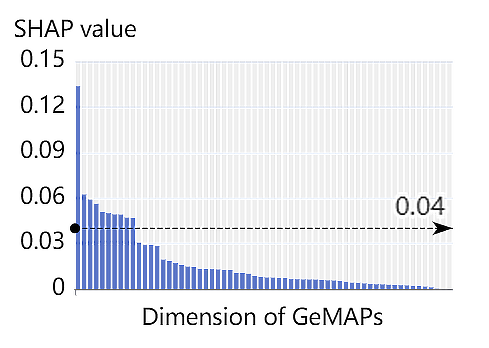
\includegraphics{images/prominent_result.png}}
	\caption{The average SHAP values (absolute value) of GeMAPs sorting from high to low. Features with SHAP values higher than 0.04 are considered prominent because of the 
sudden drop in SHAP values to the right those features. 
%These values are all absolute values to make them comparable.} 
%\KZ{Why higher than 0.04 is considered prominent? Is there any references or prev work on this? If you say this is our own def,  pls give reasons in the main text. What I observe in the fig is that the first dimension (loudness) is very high, u need to explain this. Then I see 9 features ranging from 0.4 to 0.6; then there's a sudden drop of Shapley values to below 0.03. So making the threhold at 0.04 is to account for that sudden drop?}
}%our own definition 
	%\Description {The average SHAP values of GeMAPs for prominent factors anaysis.}
	\label{fig:prominentfig} %\MYW{what do you mean sorted? ranking from high to low?}
\end{figure}



%\begin{table}[th]
%	\scriptsize
%	\centering
%	\begin{tabular}{l|c|c|c}
%		\toprule
%		Dimension & Dim Type & SHAP  & p-value\\
%		\midrule
%		\textbf{loudness\_sma3\_amean} & Energy &  0.1336 & {2.73e-83}    \\
%		\textbf{F0semitoneFrom27.5Hz\_sma3nz\_percentile50.0} & Frequency &  0.0622  & {4.76e-4}\\
%		\textbf{loudness\_sma3\_meanRisingSlope} & Energy &  0.0590  & {1.08e-7} \\
%		logRelF0-H1-A3\_sma3nz\_stddevNorm  & Frequency & 0.0561  & {0.94}\\
%		\textbf{loudnessPeaksPerSec}& Temporal  & 0.0507  & {3.75e-5}\\
%		\textbf{F0semitoneFrom27.5Hz\_sma3nz\_percentile80.0} & Frequency  & 0.0498  & {6.40e-8}\\
%		hammarbergIndexV\_sma3nz\_stddevNorm & Spectral & 0.0491  & {0.76}\\
%		\textbf{slopeV0-500\_sma3nz\_amean} & Temporal & 0.0490 & {7.37e-100}\\
%		\textbf{loudness\_sma3\_percentile80.0}& Energy & 0.0470  & {3.03e-52}\\
%		slopeV500-1500\_sma3nz\_stddevNorm& Temporal  & 0.0467 & {0.57}\\
%		\bottomrule
%	\end{tabular}
%	\caption{Details of Prominent Dimensions in GeMAPs. 
%%SHAP columns refer to the average SHAP values. 
%P-values are calculated  between the 982 barks and the speech clips. 
%Features in bold have p-value lower than 0.05, which indicates a strong correlation.}
%	\label{table:prominentfactor}
%\end{table}


\begin{table}[th]
	\scriptsize
	\centering
	\begin{tabular}{l|c|c}
		\toprule
		Dimension & Dim Type & SHAP  \\
		\midrule
		loudness\_sma3\_amean & Energy &  0.1336     \\
		F0semitoneFrom27.5Hz\_sma3nz\_percentile50.0 & Frequency &  0.0622  \\
		loudness\_sma3\_meanRisingSlope & Energy &  0.0590  \\
		logRelF0-H1-A3\_sma3nz\_stddevNorm  & Frequency & 0.0561  \\
		loudnessPeaksPerSec& Temporal  & 0.0507 \\
		F0semitoneFrom27.5Hz\_sma3nz\_percentile80.0 & Frequency  & 0.0498  \\
		hammarbergIndexV\_sma3nz\_stddevNorm & Spectral & 0.0491 \\
		slopeV0-500\_sma3nz\_amean & Temporal & 0.0490 \\
		loudness\_sma3\_percentile80.0& Energy & 0.0470  \\
		slopeV500-1500\_sma3nz\_stddevNorm& Temporal  & 0.0467\\
		\bottomrule
	\end{tabular}
	\caption{Details of Prominent Dimensions in GeMAPs. }
		%SHAP columns refer to the average SHAP values. }
	\label{table:prominentfactor}
\end{table}
%10	0.3674 2.3e-4
%3	0.0628 0.54
%16	0.0927 0.36
%29	-0.0506 0.62
%56	-0.0278 0.79
%4	0.0019 0.98
%47	-0.0620 0.55
%48	0.6177 2.0e-11
%14	0.2817 5.4e-3
%51	-0.0090 0.93
The ten prominent factors in \tabref{table:prominentfactor} fall into four categories: 
\textit{spectral}, \textit{temporal}, \textit{energy}, and \textit{frequency}, 
according to the original GeMAPS definition. Most of the prominent factors are
spectral parameters, including dimensions of HammerbergIndex and slope. 
HammerbergIndex represents the ratio of the strongest peak in the 0-2kHz region to 
the strongest peak in the 2-5kHz region, while Slope represents the linear regression slope 
of the spectral power spectrum within the given band. F0semitone-related factors describe the pitch, which is highly related to the
fundamental frequency. The factors about segment length are temporal parameters. 
The energy-related parameter loudness, which represents the sound intensity, 
is largely affected by the recording device and environment. 
%Although there is a possibility that the Japanese prefer to speak louder, it is hard to distinguish. Thus here we take it as the audio sampling difference during recording. 

%\KZ{But why the recording in Japan is siginificantly louder than the ones from the US, or vice versa?}


Considering these factors, the results show that dog vocals from two host language environments have distinctive differences in their energy distribution over frequency. In quantitative analysis, vocals from the Japanese language environment have a higher frequency than those from English.

In order to better compare the vocals with human language, we conduct a SHAP analysis on 
human speech datasets: open public language corpus CommonVoice and the host speech 
extracted from the same videos as the dog vocals. 
%\MYW{cite refs for commonvoice. Introduce this comparison in your\part{title} method section as well.}
To find out the difference between these two languages, we use xgboost as well to classify 
human speech into English or Japanese and then compute Shapley values, 
with results presented in \figref{fig:humanspeech}.

\begin{figure}[th]
	\centering
	\scalebox{0.24}{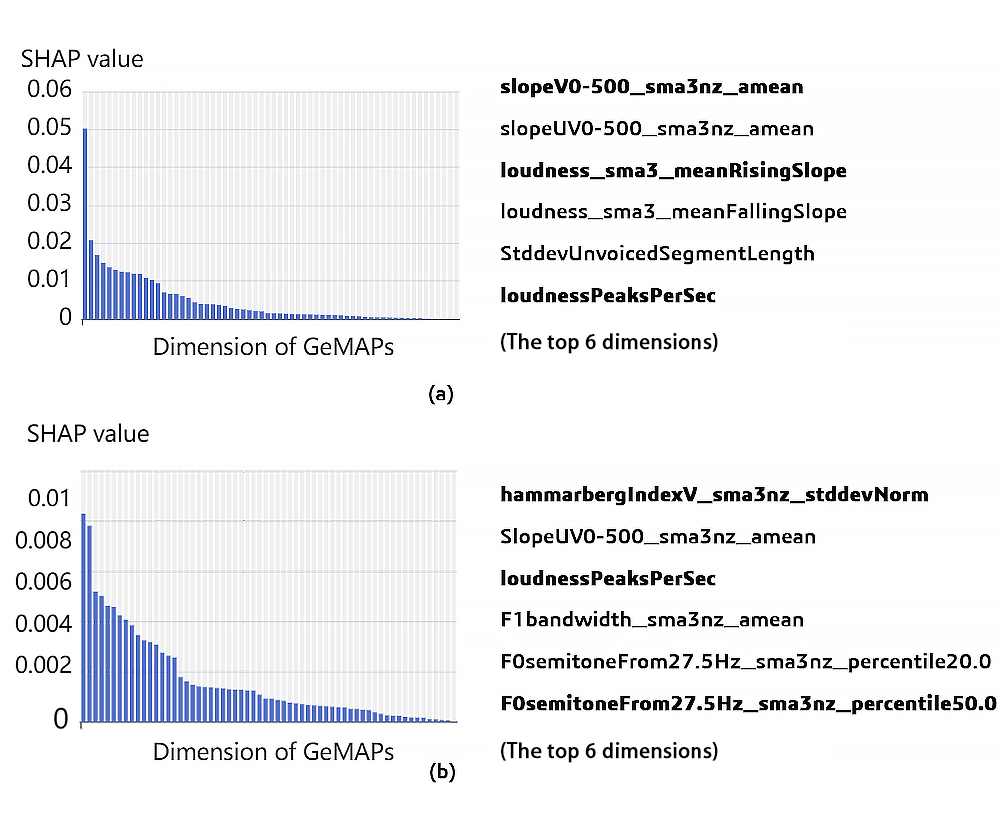
\includegraphics{images/prominent_speech.png}}
	\caption{(a) and (b) are the results of SHAP analysis ranked by descending SHAP values on open corpus and extracted human speech audios, respectively. The top six dimensions are shown on the right, 
and those that overlap with prominent factors in vocals of dogs are bolded.
%\KZ{Don't say ``SHAP value falling gradually'', instead: ``Ranked by descending SHAP values.''}
}
	\label{fig:humanspeech}
\end{figure}

% \KZ{Once we have found the common important factors between dog barks and human speeches, can we show a diagram to illustrate the correlation between dogs and human in the two communities respectively?} okok wait for me ;;;  the space is not enough now


In the human speech analysis, the difference between English and Japanese concentrates on the slope, loudness, and F0semitone. From the above, we can conclude that the difference between vocals coming from different host language environments is mainly related to frequency. In the meantime, from our analysis of prominent acoustic factors, the vocalsvocals  of dogs and 
voices of humans share several common prominent factors, suggesting that the 
host human language have a correlation with the vocals of dogs.
\begin{table*}[th]
	\small
	\centering
	\begin{tabular}{l|c|c|c|c}
		\toprule
		\multirow{2}*{Dimension} &
		\multicolumn{2}{c|}{With Host Speech} & \multicolumn{2}{c}{With Random Speech}\\
		\cline{2-5} 
		& Pearson Coefficient & \textit{p}-value & Pearson Coefficient &  \textit{p}-value \\ \hline
		\textbf{loudness\_sma3\_amean}& 0.537& 	2.73e-83& 	0.025 & 0.405  \\ 
		\textbf{F0semitoneFrom27.5Hz\_sma3nz\_percentile50.0} & 0.105& 	4.76e-4	& -0.012 &	0.691\\ 
		\textbf{loudness\_sma3\_meanRisingSlope} & 0.159& 	1.08e-7& 	0.043& 	0.155 \\
		logRelF0-H1-A3\_sma3nz\_stddevNorm & 0.002 & 0.941	& 4.25e-4 & 0.989\\
		\textbf{loudnessPeaksPerSec} & 0.124 & 3.75e-5 & 1.20e-3 & 0.968\\
		\textbf{F0semitoneFrom27.5Hz\_sma3nz\_percentile80.0} & 0.162 & 6.40e-8 & -0.011	& 0.714\\
		hammarbergIndexV\_sma3nz\_stddevNorm & 9.13e-3 & 0.762	& 6.47e-3 & 0.830\\
		\textbf{slopeV0-500\_sma3nz\_amean}& 0.580	& 7.37e-100 & 	0.029& 	0.334\\
		\textbf{loudness\_sma3\_percentile80.0} & 0.436 & 3.03e-52 & 	0.030 & 	0.322\\
		slopeV500-1500\_sma3nz\_stddevNorm & 0.017 & 0.573& -4.40e-3  & 0.884\\
		\bottomrule
	
	\end{tabular}
	\caption{The correlation analysis is on two groups of data. In the first group, the analysis is on the correlation between dog vocals and their host speech, in the second group the correlation is between dog vocals and random speech. The dimensions of high correlation with p-value lower than 0.05 are bold.}
	\label{table:prominentpearson}
\end{table*}


Furthermore, to ascertain the correlation between vocals and speech more 
directly besides the overlap of their prominent factors, we calculate the 
Pearson's correlation between the two from the same videos 
in the ten prominent dimensions selected (\tabref{table:prominentpearson}). 

\subsubsection{Language Speed Comparison}
\label{sec:prominentfactor1}
Dog vocals under English and Japanese host language environments differ not only in these 
acoustic dimensions above, but a more intuitive dimension: \textit{speed}.

A formal measure of the speed of speech is the number of syllables in 
a given time duration. For speech from the same video as the dog voices, 
we apply an automatic speech 
recognition (ASR) model in Whisper~\cite{radford2022robust}, one of the state-of-the-art ASR models 
which smoothly transcribes the extracted speech into either English or Japanese texts. 
%\MYW{we need to report the WER, word error rate or say that whisper is one of the SOTA asr models} 
At the same time, CommonVoice already provides corresponding texts for their audio.
The segmentation of text into sequences of syllables is done by some subfunction of 
\textit{eSpeak}~\cite{duddington2012espeak}, which is a compact open source software speech synthesizer for 
English and other languages.
However, as there is no concept of ``syllable'' nor alphabet for Shiba 
Inu barks, 
we adopt another similar way for syllablizing dog clips. The dog clips are 
divided into sequences of syllable-like units according to an oscillator-based 
algorithm~\cite{rasanen2018pre}.
\begin{figure}[th]
	\centering
	\scalebox{0.20}{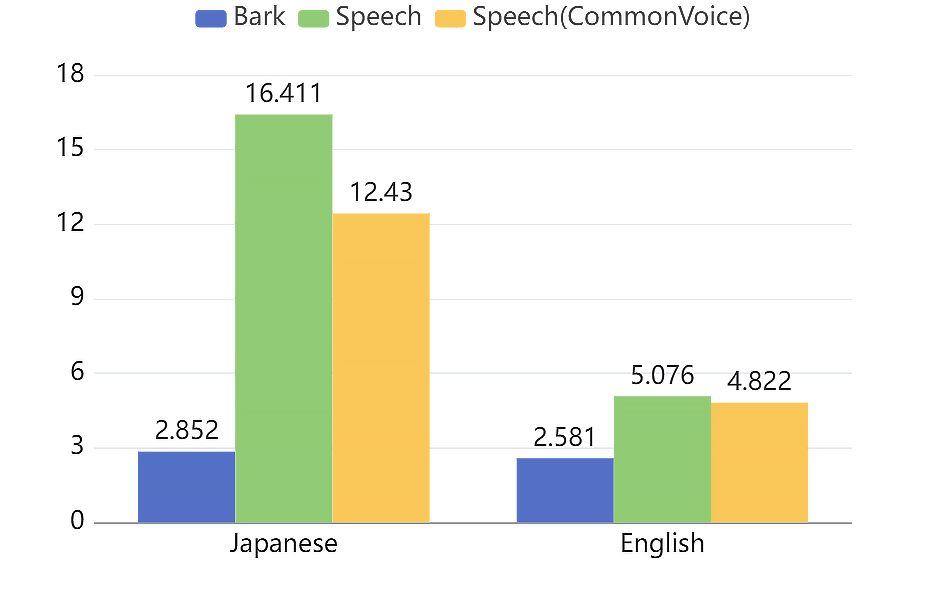
\includegraphics{images/speed.png}}
	\caption{The speed comparison for barks, host speech from same video and speech from CommonVoice.}
	\label{fig:speedcomparison}
	%\Description {The speed comparison for barks, speech from same video and speech from CommonVoice.The japanese speak faster, so do the dogs in japanese environment.}
\end{figure}

The number of syllables or syllable-like units per second is shown 
in \figref{fig:speedcomparison}.  We make the following discoveries: 
%\KZ{Rewrite the next two paragraphs. Bad English.} T T ok ok
First, dog vocals from Japanese environment and Japanese human speech clips 
are generally faster than dog vocals from English environment and English speech clips. 
This suggests that when it comes to speed, there is a correlation between dog
vocals and human speech. %\KZ{is the japanese dogs significantly faster than english dogs?
%that is, 2.852 vs 2.584 syllables per sec?  can we do a t-test here?}
% JY: t-test only for data more than two.
Second, it appears that human speech in EJShibaVoice dataset is faster than
that of CommonVoice.  %\KZ{What do you mean by scaling? They are actually similar 
%after scaling.} 
The difference in speed can be attributed to the 
recording style of CommonVoice, which tends to be slower than typical speech.

Here we illustrate the spectrograms of two typical dog vocal samples from the 
two language environments in~\figref{Fig.sample}. 
It is clear that in the same time length, the vocal under Japanese language environment has more syllable-like units than that under English language environment while the frequency of those vocals 
in the English environment is closer to the low-frequency region.

\begin{figure}[th]
	\centering
\begin{subfigure}[t]{0.49\columnwidth}
        \centering
        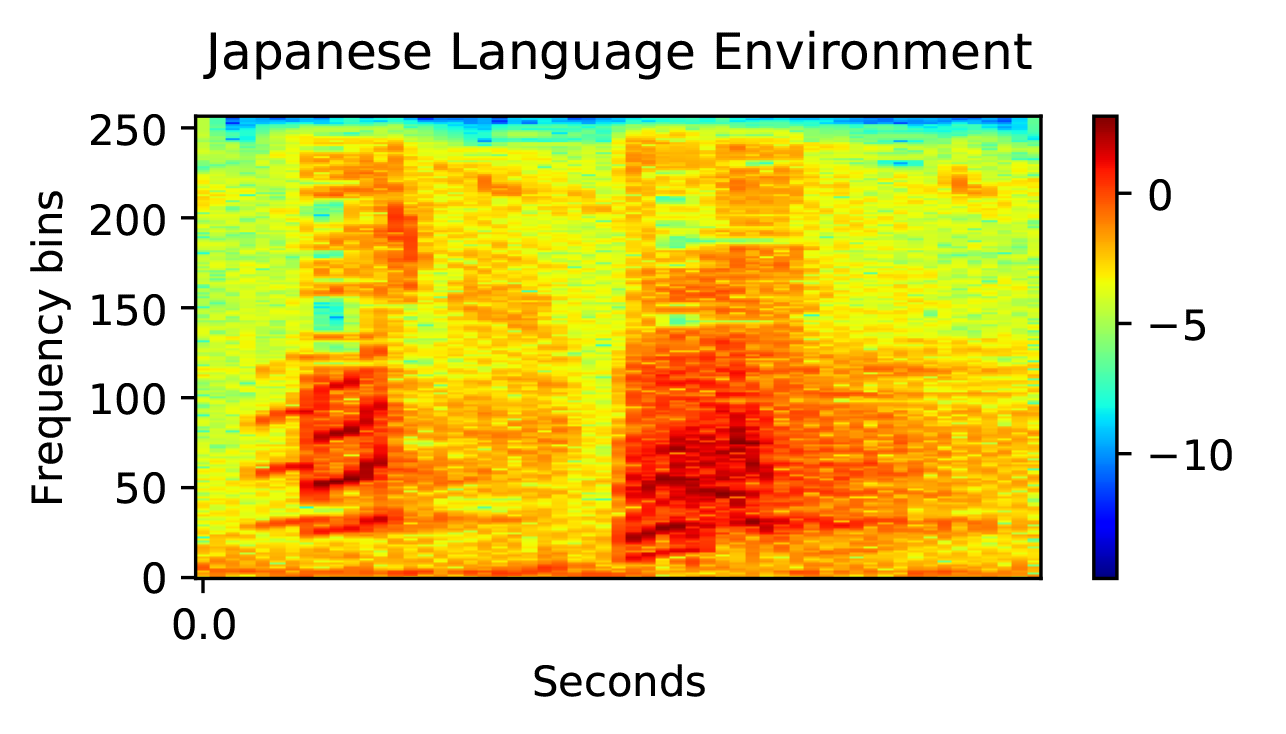
\includegraphics[width=\textwidth]{dog_spec_ja_1.png}
        \caption{A Bark under Japanese Env.}
        \label{fig:subja}
\end{subfigure}
\begin{subfigure}[t]{0.49\columnwidth}
        \centering
        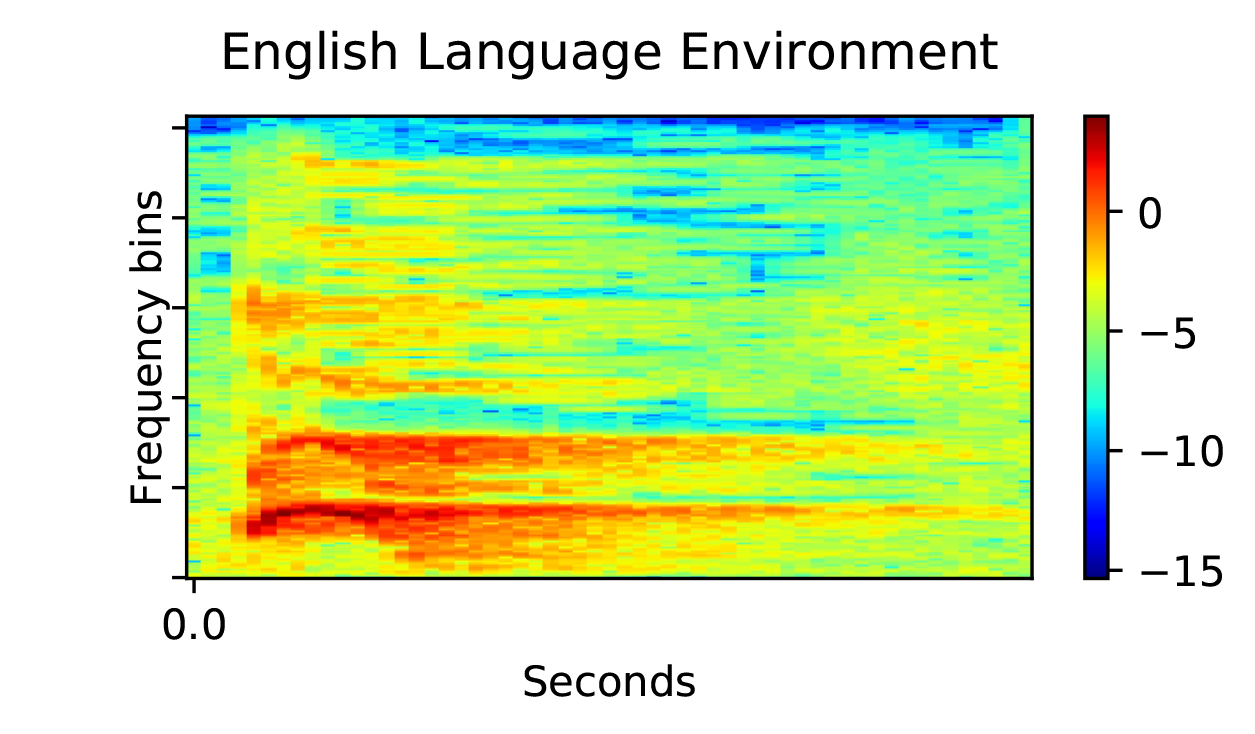
\includegraphics[width=\textwidth]{dog_spec_en_1.png}
        \caption{A Bark under English Env.}
        \label{fig:suben}
\end{subfigure}
	\caption{The spectrogram of two audio samples which are from different language environmentsand similar situations.}
	\label{Fig.sample}
\end{figure}

%\subsection{Human Evaluation}
%In addition, we conducted a subjective evaluation by humans to bolster our results. The evaluation contains 20 pairs of vocals from different host language environments (En-Ja and Ja-En pairs), and we invited 30 normally-hearing college students to answer a series of questions after listening to each pair of vocals. 
%They were asked to tell whether the vocals in a pair were from the same or different language environments, 
%and if different, what is the most significant factors among the four options: speed, pitch, 
%non-voice segment length (pauses), and loudness. 
%This experiment collected 600 answers in total. Results indicated that 59.00\% 
%of the participants can distinguish differences between a pair, and 79.09\% agree that 
%the difference lies in pitch, which is the auditory perceptive expression of frequency. 
%The subjective evaluation results coincide with our statistical analysis. \MYW{This is difficult to interpret, that humans can barely distinguish country origin, is it still necessary to include?} \KZ{Maybe instead of saying asking
%the annotators to distinguish if the pair comes from two diff lang enviroment,
%ask them if the pair comes from the same family, or even if the pair comes from
%the same dog? This might be easier to listen for us human beings?}


\subsection{Summary of Findings}

Through all the above analysis, we can find that \textbf{the key accoustic features that distinguish Shiba Inus from two language environments are frequency and speed, which correlate well with human speech.}

%\KZ{You need to give a straight answer to your research question 2, what are key features
%that distinguish between Japanese and English dogs? You should bold this answer 
%just like in prev section.}

%0.537285079	2.73E-83	0.025114482	0.405331422
%0.105176365	0.00047578	-0.011997723	0.691012547
%0.159345952	1.08E-07	0.04295332	0.154551349
%0.002236163	0.940946	0.000425422	0.988755288
%0.123958131	3.75E-05	0.001200178	0.96828435
%0.16214011	6.40E-08	-0.011072311	0.713752752
%0.00913266	0.762226725	0.006468961	0.830305739
%0.579943095	7.37E-100	0.029178255	0.333624609
%0.435957276	3.03E-52	0.029890759	0.321950071
%0.016995079	0.573392109	-0.004395997	0.884210585



%Literature
Our findings corroborate with previous literature~\cite{doi:10.1126/sciadv.aaw2594, graham2014fundamental} that the syllable speed of Japanese surpasses that of English and many other languages. At the same time, the frequency of Japanese is relatively higher than that of English. All these findings show that the vocals under English and Japanese language environments are different and in two dimensions of frequency and speed. To explain in detail, English dog vocals at a lower frequency than Japanese dogs, but Japanese dog vocals faster than English dogs. The same phenomenon can be observed with human speakers of these two languages. %And furthermore, these findings match with the literature.

%In the end, I would like to see a summary of findings that provides answers to the two research questions. For the second questions, I would like to see that you say:The key accoustic features that distinguish Shiba Inus from two language environmentsare frequency and speed. Specifically, English dogs bark at a higher frequency thanJapanese dogs, but Japanese dogs barks faster than English dogs.The same phenomenon can be observed with human speakers of these two languages.And furthermore, these findings corroborate with the literature~\cite{doi:10.1126/sciadv.aaw2594,graham2014fundamental}.

% \KZ{What are the composition ofthese human participants?}

% \MYW{human studies sound weird..maybe stick to The subjective evaluation results echo our statistical analysis}

%%%%%%%%%%%%%%%%%%%%%%%%%%%%%%%%%  specific evaluation name %%%%%%%%%%%%%%%%%

\subsection{Human Evaluation on Acoustic Features}
Alongside acoustic analysis, we assess cross-linguistic dog vocals via surveys. We pick 20 vocal pairs with distinct language settings from \secref{sec:method}. Each of the 20 questionnaires, given to 30 participants, makes 600 in total. Pair sequence is randomized. When spotting differences, participants gauge from four dimensions below%\MYW{this sentence reads weird, rephrase, ascertain the diffference between two clips?}
: (1)urgency, which represents the speed (2)pitch (3)duty ratio, which is the ratio of the duration of the voiced segments to that of the unvoiced segments (4)loudness. 
%\MYW{what does urgency, duty ratio mean?}
%It should be noted that for each dimension, people can only choose which clip performs higher on this dimension or there is no obvious difference. 

Among four above dimensions, 74.01\%, 79.09\%, 67.23\% and 63.56\% of the questionnaires which says that there are differences between the two clips report dimension difference respectively. This shows that from a human perspective the differences are most revealed by pitch, which is highly frequency related. This is in line with our acoustic analysis.


%, it's higher than 74.01\%, 67.23\%, 63.56\% for the other three dimensions respectively\MYW{rewrite this sentence, unclear statement}. 

%\KZ{Maybe we can show the spectrum of human voices between jap and english as well since we have some space?}%reply: there is no room for spectrum between jap and english.
% \MYW{Adding in the human perception analysis? Indicating 1)humans can tell the difference between dog barks from different host languages 2)the prominent factors are in line with our acoustic analysis}

\subsection{Restrictions}
Compared to previous studies, we adopt a first-of-its-kind method of collecting data from the  Internet. Some may argue that former studies have a more controllable environment to eliminate confounding factors. However, it is very unlikely to cultivate exactly the same growing environment as subjectivity always exists. On the contrary, with the large amount of data from various families, we can remedy the confounding factors in a statistical way. Our pipeline is hence beneficial as we can scale up the data in the future and further validate our argument.
%%%%%%%%%%%%%%%%%%%%%%%%%%%%%%%%%%%%%%%%%%%%%%%%%%%%%%%%%%%%%%%%%%%%%%%%% add a section: limitation + about the confounding factors(1. their methods impossible 2. our methods how to remedy the bias 3. we have possibility to scale up the data) %%%%%%%%%%%%%%%%%%%%%%%%%%%%%%%%%%%%%%%%%%%%%%%%%%%%%%%%%%%%%%%%%%%%%%%%%%%%%%%%%%%%%%%%%%%%%%%%%%%%%%%%%%%%%%%%%%%%%%%%%%%%%%%%%%%%%%%%%%%%%%%%%%%%
